\chapter{Introduction}

% Trends of the electronic field is size reduction
La miniaturisation des technologies de circuits intégrés se poursuit de nos jours avec une intégration toujours plus massive des fonctions électroniques.
La réduction de taille est possible en utilisant des technologies intégrées plus fines.
Une technologie définie les dimensions et les procédés nécessaires à la fabrication du circuit intégré et à la réalisation de ses briques de conception.
Toute technologie possède une taille caractéristique \textlambda{} représentant la plus petite dimension possible pour une grille de transistor.
La valeur de \textlambda{} est essentielle et conditionne fortement la taille du circuit final, sa consommation et ses performances.
Jusqu'à présent, la loi de Moore a prédit avec succès que \textlambda{} serait réduit d'un facteur deux tous les dix-huit mois.
Le domaine automobile se conforme à cette tendance, en utilisant récemment des nœuds technologiques à 16 nm (Fig. \ref{fig:nxp-techno-increase}) \cite{evolution_technologies} normalement utilisés dans des applications moins sévères.

% Benefits of size reduction
La diminution du \textlambda{} se traduit par l'intégration d'un plus grand nombre de fonctions pour une surface de silicium donnée.
Le facteur principal du coût dans la réalisation d'un circuit intégré est l'aire occupée sur silicium.
La diminution de taille permet de réduire la surface nécessaire a la réalisation du circuit et donc son coût unitaire.
A taille constante, des circuit intégrés plus denses peuvent embarquer plus de fonctionnalités et ont des performances plus élevées.
La réduction de poids des modules électroniques pour l'automobile ou l'aéronautique permet de diminuer la consommation de carburant, de réduire les coûts et l'impact sur l'environnement.

\begin{figure}[!h]
  \centering
  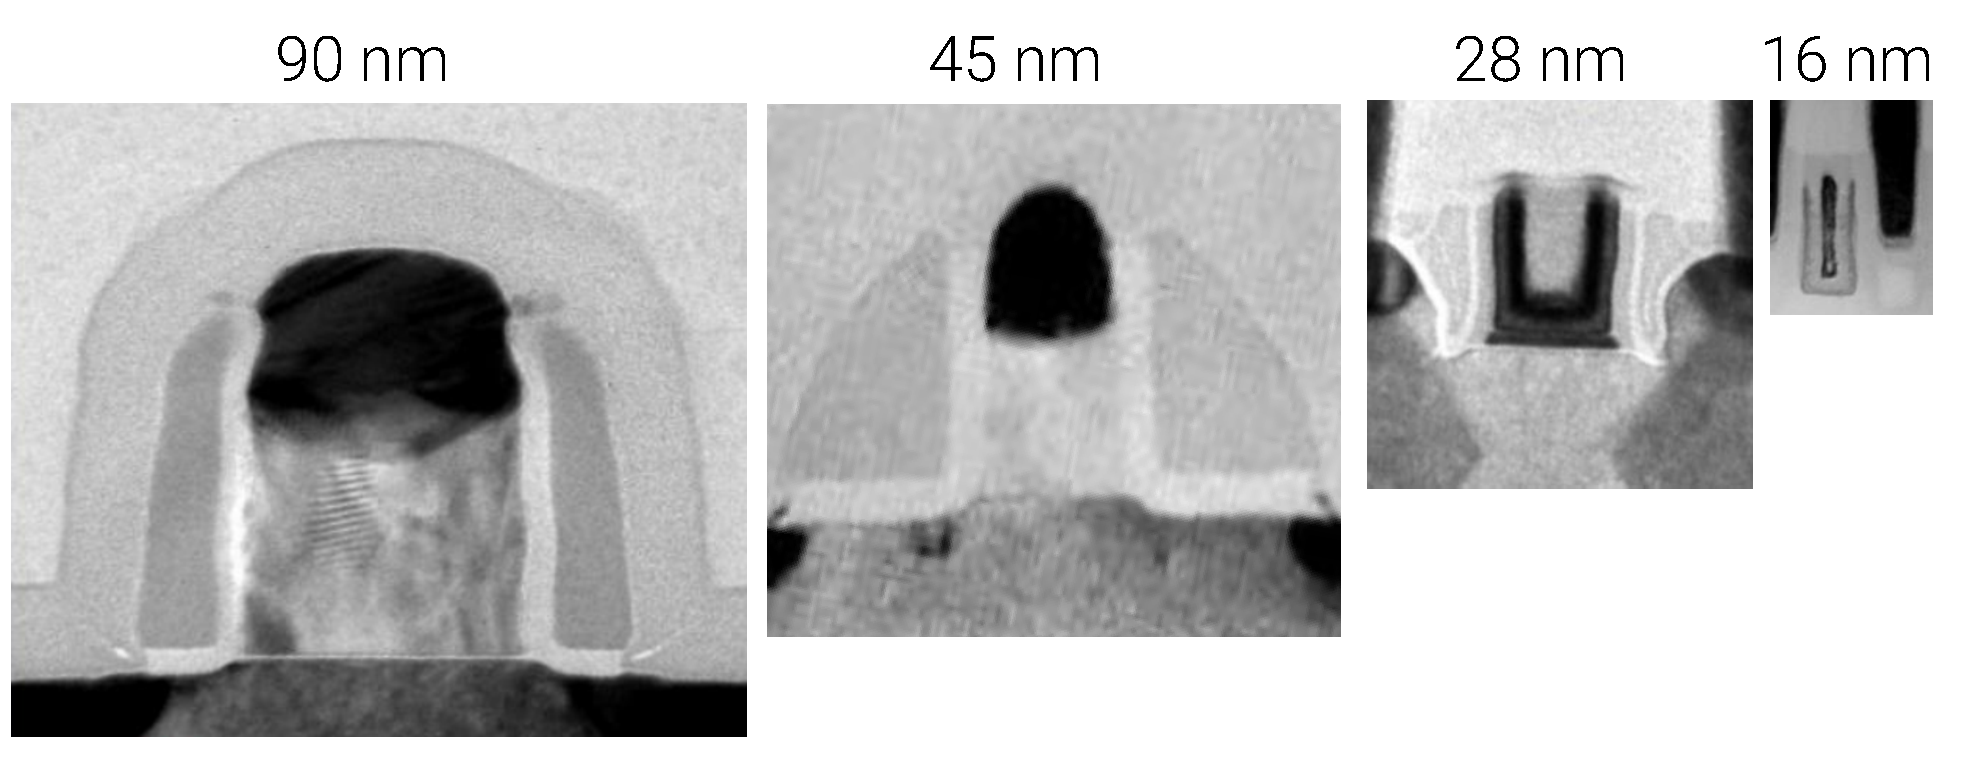
\includegraphics[width=\textwidth]{src/1/figures/technology_evolution.pdf}
  \caption{Évolution actuelle des nœuds technologiques de NXP \cite{evolution_technologies}}
  \label{fig:nxp-techno-increase}
\end{figure}

% Side effects of size reduction
En réduisant la taille des circuits, les épaisseurs des matériaux isolants dans le procédé technologique sont également diminués.
C'est le cas des oxydes nécessaires à la réalisation des grilles de transistors par exemple.
Une épaisseur d'isolant plus fine tolère des différences de potentiel moins élevées.
Au delà, un claquage de l'isolant se produit rendant généralement le composant inutilisable.
Les seuils de tolérances en tension et courant deviennent donc plus petits, et de manière générale la réduction de taille s'accompagne d'une augmentation de la fragilité et de la sensibilité des circuits intégrés.
La surface de silicium nécessaire à la protection des cœurs de circuits occupe une plus large part de l'aire totale d'un produit  \cite{evolution_technologies} et donc du coût.

% Another trend in automotive - more electronic functions
De nouvelles tendances propres au domaine automobile voient le jour depuis quelques années.
Les véhicules autonomes sont en très fort développement et commencent à faire leur apparition sur les routes.
Ces type de fonctionnalité prends des décisions et applique des actions critiques sur le véhicule en temps réel.
Elles interagissent avec des équipements essentiels du véhicule tels que la direction ou les freins.
A terme, elles promettent une augmentation de la sécurité des usagers d'un véhicule.
La contrainte temps-réel sur ce type de système électronique est très importante, car il est nécessaire de garantir leur fonctionnement normal quel que soit les perturbations auxquelles ils vont être exposés.

% Harsh environment in the automotive field
L'environnement automobile est très sévère pour les composants électroniques.
Un moteur en fonctionnement génère de la chaleur et des vibrations.
Durant toute sa vie, un véhicule est exposé à de larges cycles thermiques.
Les contacts électriques, les soudures et les connexions vieillissent plus rapidement.
De plus, les systèmes électroniques sont exposés à une large plage de stress électriques.
Quand le moteur est allumé, la tension de batterie chute fortement à cause de l'appel de courant créé par le démarreur.
Cette variation très brutale peut affecter ou endommager les modules.
La déconnexion d'une batterie génère des décharges brutales de câbles dans les systèmes électroniques, pouvant entraîner leur destruction.
Il existe également une autre famille de perturbations électriques appelée décharges électrostatiques (ESD - ElectroStatic Discharge), auxquelles sont exposés tous les systèmes électroniques en général.
Dans l'automobile, ces phénomènes sont particulièrement violents.
% What is an ESD
Une décharge électrostatique est un transfert de charge soudain entre deux objets de différente charge.
C'est le résultat d'une accumulation de potentiel électrostatique.
La décharge se produit lorsque la différence de potentiel est suffisamment large.
L'amplitude de tels événements peut atteindre couramment plusieurs milliers de volts et des dizaines d'ampères.
D'après une étude du fabricant de véhicules Renault \cite{Renault-esd}, il est estimé que les composants électroniques automobiles sont exposés 10000 fois à des décharges pendant leur vie.
Les circuits intégrés sont particulièrement vulnérables \cite{impactESDsemiconductors} et nécessitent des mesures de protection particulières.

% Architecture systemes automobiles
L'architecture des systèmes électriques et électroniques dans un véhicule est assez complexe.
Une voiture est constituée d'une multitude de modules électroniques interconnectés par des câbles.
Pour communiquer et fonctionner correctement, les modules électroniques ont besoin d'une bonne référence de masse.
Ceci est assuré par la carcasse métallique du véhicule, et les modules ainsi que la batterie y sont tous connectés via des câbles.
En statique et à basse fréquence, cette référence est très bonne car la carcasse et les câbles sont très peu résistifs.
A haute fréquence, ces câbles ont un caractère inductif.
Ils s'opposent aux variations de courant et présentent des différences de potentiel importantes.
Par conséquent, la connexion de masse est dégradée et des perturbations locales peuvent affecter un module en décalant sa référence par exemple.
Par nature, les décharges électrostatiques sont des évènements très courts de forte amplitude, avec donc un contenu spectral important à haute fréquence.
Elles sont donc susceptibles de perturber localement des systèmes électroniques dans un véhicule.
Pour contrecarrer ce problème, les modules sont conçus pour être robustes, mais il reste difficile de garantir leur immunité face à des phénomènes aussi violents que des ESDs.

\begin{figure}[!h]
  \centering
  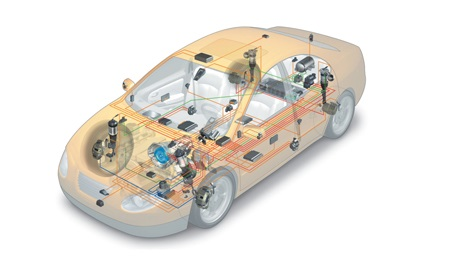
\includegraphics[width=0.8\textwidth]{src/1/figures/systemintegration_01_uv-data.jpg}
  \caption{Architecture des systèmes électroniques dans un véhicule (Crédit: Continental \cite{car-architecture})}
  \label{fig:car-architecture}
\end{figure}

% Fiabilite vis a vis des ESD
Dans le domaine des décharges électrostatiques, il y a deux types de défaillances à considérer.
La défaillance matérielle ou "hard-failure" est le résultat de la destruction d'un composant.
Elle peut avoir lieu par rupture des oxydes lorsque la tension a dépassé un niveau maximum ou par échauffement lorsque le courant circulant est trop important.
Deux exemples de casse sont donnés Fig. \ref{fig:esd-failures}.
Récemment, un deuxième type de défaillance commence à être étudié.
Les défaillances fonctionnelles ou "soft-failure" prennent la forme d'une perturbation d'une fonction électrique intégré.
Elles peuvent être causées par toutes sorte de perturbations électriques et en particulier par des décharges électrostatiques.
Plusieurs niveaux de sévérité existent.
Par exemple, la perturbation d'un système d'airbag peut l'empêcher de se déclencher en cas de besoin, ce qui est bien plus critique qu'un problème d'affichage sur le tableau de bord.

\begin{figure}[!h]
  \centering
  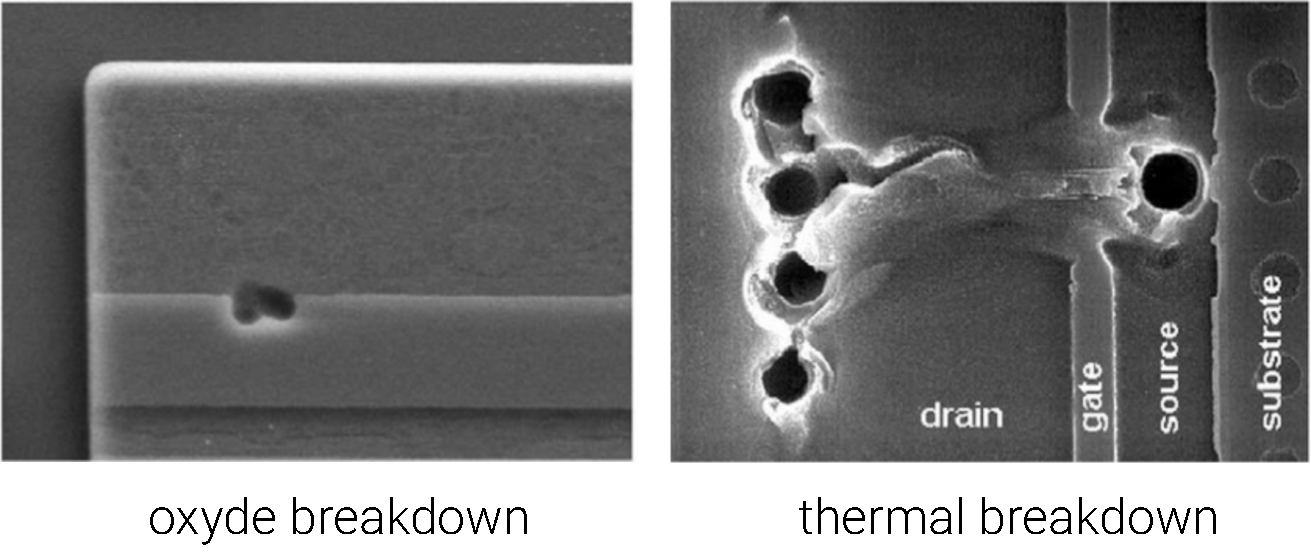
\includegraphics[width=0.8\textwidth]{src/1/figures/esd_failures.pdf}
  \caption{Types de défaillances matérielles causées par des ESD}
  \label{fig:esd-failures}
\end{figure}

% Comment predire ces defaillances fonctionnelles
Les premiers travaux sur ce sujet ont été publiés par F. Caignet et N. Lacrampe en 2007 \cite{LacrampeTransientImmunity}.
Également, de nombreuses recherches sur les défaillances au niveau système ont été publiées pendant les symposia EOS/ESD 2012 \cite{soft-error-esd-1,SDRAMCase,mixedModeESDSims} et 2013 \cite{softFailSubsystem, powered-tlp-soft-fail}.
Le standard IEC 62433-6 \cite{iec62433-6} encore en phase d'élaboration cherche à formaliser des méthodes pour l'analyse et la prédiction de fautes fonctionnelles.
L'analyse de la littérature montre que les recherches sur les défaillances fonctionnelles liées aux décharges électrostatiques restent focalisées au niveau système.
Dans ce document, la recherche et l'analyse de faiblesses fonctionnelles a lieu plus bas dans la hiérarchie, au niveau circuit-intégré.
Il est nécessaire de comprendre comment une fonction intégrée est perturbée par une décharge, afin de pouvoir la protéger correctement dans son environnement de fonctionnement.
Plusieurs approches sont explorées dans ce document.
Une méthode de modélisation des éléments au niveau système est améliorée a partir des travaux précédents sur le sujet \cite{phd-lacrampe, phd-monnereau}.
Elle permet de déterminer quelle fraction d'une décharge appliquée sur un système est réellement vue par un circuit intégré.
Des méthodes de mesure pouvant être intégrées sur silicium sont aussi proposées, afin d'acquérir plus de données sur le problème.
Un capteur de courant sur puce, des détecteurs de surtension et sous-tension ainsi qu'une chaine de communication ont été développés et fabriqués sur une puce de test.
Des méthodes de modélisation de fonctions intégrées, à l'intérieur de la puce, ont été proposées.
Elles restent au stade de prototype mais offrent un début de réponse pour aborder les problèmes de défaillances fonctionnelles au niveau puce.
L'objectif est de réduire la complexité du problème afin de pouvoir l'aborder de manière modulaire, en étudiant d'une part les blocs d'un circuit individuellement, puis en considérant leurs interactions.

% Presentation des chapitres
%
Cette introduction (chapitre 1) a présenté de manière succincte les points clés et les enjeux du sujet de recherche.

Le chapitre \ref{chap:1} fournit en détail les notions essentielles à la compréhension de la problématique.
Il explique comment les décharges électrostatiques apparaissent et comment elles sont reproduites en laboratoire.
Une revue de l'état de l'art est faite sur l'analyse des pertes de fonctionnalités dues à des décharges.

%
La chapitre \ref{chap:2} présente un méthode de modélisation pour simuler la propagation de décharges électrostatiques jusqu'au composant.
Une librairie de modèles est construite, ensuite assemblés ensemble pour reproduire le système à simuler.
Un générateur de stress utilisé dans le laboratoire de test à NXP est modélisé pour illustrer la méthode.
Un nouveau générateur de stress 50 \textOmega{} appelé TLP-HMM est ensuite proposé, reproduisant une forme d'onde standardisée.
Il présente plusieurs avantages sur les générateurs conventionnels, tels que le fait d'être blindé et de ne pas perturber les circuits par émission électromagnétiques, ainsi que d'offrir des niveaux de reproductibilité des tests excellents.
Ce générateur est particulièrement intéressant pour effectuer des tests de décharge sur des circuits intégrés alimentés.

%
Un cas de défaillance fonctionnelle est ensuite présenté dans le chapitre \ref{chap:3}.
Tout d'abord, des mesures sont effectuées de manière externe sur le circuit intégré sous test.
La signature de la défaillance est expliquée.
Un circuit intégré de test est développé et fabriqué, contenant des structures spéciales pour mesurer les perturbations directement sur le silicium.

%
Ces travaux ont aussi été orientés vers la recherche de nouvelles méthodes de simulation.
L'objectif est de détecter plus facilement et rapidement des défaillances fonctionnelles, en utilisant les outils existants de simulation.
Différentes méthodes sont présentées dans le chapitre \ref{chap:4}.
La première méthode permet une caractérisation individuelle de blocs dans une fonction intégrées afin de construire un modèle.
Ces modèles peuvent ensuite être chaînés pour déduire de manière immédiate la robustesse de la fonction complète sans effectuer de simulation supplémentaire.
La seconde méthode cherche à créer un modèle boite-noire d'une fonction intégrée, c'est à dire un modèle faisant abstraction de la conception interne.
L'objectif est de permettre une simulation au niveau système avec le circuit intégré sans connaitre le design interne.
Elles ont chacune des applications différentes, mais peuvent s'avérer complémentaires pour concevoir des circuits robustes, que ce soit au niveau système ou circuit intégré.

%
Enfin, la conclusion résume les travaux effectués et présente des axes de recherche futurs.
